	\begin{figure}[!h]
		\centering
 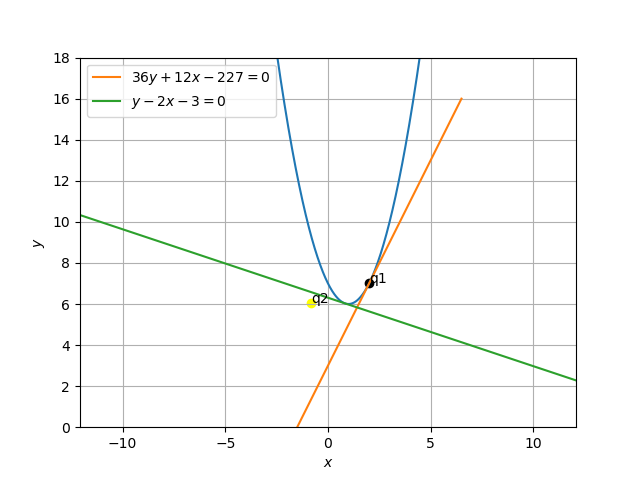
\includegraphics[width=\columnwidth]{chapters/12/6/3/15/figs/conic.png}
		\caption{}
		\label{fig:12/6/3/15}
  	\end{figure}
The parameters of the given conic are
\begin{align}
\vec{V} =\myvec{
	1 & 0\\
	0 & 0
	},
    \vec{u}=-\myvec{
	1 \\
	\frac{1}{2}
	},
    f=7
    \end{align}
\begin{enumerate}
	\item In this case,  the normal vector
		\begin{align}\vec{n}_1 = \myvec{2 \\ -1}\end{align}
			Since 
$\vec{V}$ is not invertible,  
		%Then given the normal vector \begin{align}\vec{n}\end{align}\, 
	the point of contact is given by 
\eqref{eq:conic_tangent_q_eigen} resulting in 
		%the matrix equation
\begin{align}
\myvec{\myvec{-1 \\ -\frac{1}{2}} + \frac{1}{2}\myvec{2 \\ -1}^{\top} \vspace{0.3cm}\\ \myvec{
	1 & 0\\
	0 & 0\\
	}} \vec{q}_1 = \myvec{-7 \vspace{0.3cm}\\ \frac{1}{2}\myvec{2 \\ -1} - \myvec{-1 \\ -\frac{1}{2}}}
\end{align}
By solving the above equation, we can get the point of contact as
    \begin{align}
  \vec{q}_1=\myvec{
	2 \\
	7 \\
	}
\end{align}
The 
tangent equation is then obtained as
\begin{align}
      \vec{n}_1^{\top}(\vec{x}-\vec{q}_1) = 0
  \\
	\implies  \myvec{2 & -1}\vec{x}+3 = 0
\end{align}
\item 
In this case, 
		\begin{align}\vec{n}_2 = \myvec{1 \\ 3} \end{align}
resulting in 
\begin{align}
\myvec{\myvec{-1 \\ -\frac{1}{2}} + -\frac{1}{6}\myvec{1 \\ 3}^{\top} \vspace{0.3cm}\\ \myvec{
	1 & 0\\
	0 & 0\\
	}} \vec{q}_2 = \myvec{-7 \vspace{0.3cm}\\ -\frac{1}{6}\myvec{1 \\ 3} - \myvec{-1 \\ -\frac{1}{2}}}
\end{align}
    \begin{align}
	    \text{or, }  \vec{q}_2=\myvec{
	\frac{5}{6}
\\
	\frac{217}{36}
	}
\end{align}
The tangent equation is
\begin{align}
      \vec{n}_2^{\top}(\vec{x}-\vec{q}_2) = 0
      \\
	\text{or, }    \myvec{1 & 3}\vec{x}= \frac{227}{12}
\end{align}
\end{enumerate}
		See \figref{fig:12/6/3/15}.
